\documentclass[a4paper]{article}       % Default text size and document class

% Format -----------------------------------------------------------------------------
\usepackage[                    % To set up the page
  a4paper,                        % A4 paper
  width=160mm,                    % Text body width
  top=25mm,bottom=25mm,           % Top and bottom margins
  bindingoffset=6mm               % Offset of left and right pages for printing
  ]
 {geometry}
\usepackage{setspace}           % So set spacings (e.g. line height)
  \onehalfspacing                 % Sets line width to 1.5
%\usepackage{sectsty}            % To control sectional headers
%  \chapternumberfont{\huge}       % Set size of chapter number
%  \chaptertitlefont{\huge}        % Set size of chapter title 

\usepackage{multicol}           % Writes in multiple columns
\usepackage{wrapfig}
\usepackage{lipsum}             % Inserts blind text for previewing
\usepackage{placeins}           % adding float barriers 
\setlength{\parindent}{0pt}     % remove indentation for new paragraphs

% Language ---------------------------------------------------------------------------
\usepackage[english]{babel}     % To enable language support other than us english
\usepackage[babel]{csquotes}    % Omits spell checking in quotations

% Images, long tables & append pdf pages ---------------------------------------------
\usepackage{float}              % Enables some options for image placement
\usepackage{graphicx}           % To include graphics
\usepackage{                    % Long table stuff
  csvsimple,                      % So a csv can be converted to a table
  longtable,                      % To make long tables
  booktabs                        % To page break long tables properly
  }
\usepackage{pdfpages}           % Appends pdf pages
\usepackage{xcolor}

% Custom fancy image caption ---------------------------------------------------------
\usepackage{caption}
  \captionsetup[figure]{labelsep=space}
%  \captionsetup[table]{labelsep=space}
  \newcommand{\mycaption}[2]{\caption[#1]{\textbar\,\textbf{#1} #2}}

% Math and code support -----------------------------------------------------------------------
\usepackage{amsmath, amsfonts}  % For fancy math
\usepackage[separate-uncertainty = true]{siunitx} % for SI units
\sisetup{detect-all}
\usepackage{xcolor}
\NewDocumentCommand{\codeword}{v}{%
\texttt{\textcolor{black}{#1}}%
}
% Citation setup ---------------------------------------------------------------------
\usepackage[]{hyperref}         % To make clickable links
  \hypersetup{hidelinks,}         % To draw no boxes around the links
\usepackage[                    % Citation setup  
    backend=biber,                % Citation backend
    style=apa,           % Citation format
    % minbibnames=1,
    % maxbibnames=99,
    %maxnames=2,                 % Max number of names displayed in text
    %sortlocale=de_DE,             % Sorts by german conventions (ß = ss)
    %natbib=true,                   % Enables \citep and \citet. Use \parencite and \textcite in future
    url=false,                    % Disaples url
    doi=true,                     % To print the doi
    eprint=false                  % Disables link to eprint (?)
]{biblatex}
\DeclareDelimFormat[parencite]{finalnamedelim}{\addspace and\space} % disabels & and uses 'and'

\DeclareDelimFormat[bib,biblist]{finalnamedelim}{\addspace and\space} % disabels & and uses 'and' in the bibfile

\addbibresource{chirpdetection.bib} % Where the bibliography file is
\renewcommand{\familydefault}{\sfdefault}
\usepackage{tgheros}
\usepackage{wrapfig}
%\setlength{\marginparwidth}{1.8cm}
\usepackage[disable]{todonotes}
%\DeclareUnicodeCharacter{0301}{\textcolor{red}{*************************************}} % for finding unicode erros in the pdf 


\setlength\bibitemsep{2\itemsep} 

% Abstract title same size as sectional headers --------------------------------------
% see here: https://tex.stackexchange.com/questions/366169/how-to-change-font-size-for-abstract-title
\makeatletter
\renewenvironment{abstract}{%
    \if@twocolumn
      \section*{\abstractname}%
    \else %% <- here I've removed \small
      \begin{center}%
        {\bfseries \Large\abstractname\vspace{\z@}}%  %% <- here I've added \Large
      \end{center}%
      \quotation
    \fi}
    {\if@twocolumn\else\endquotation\fi}
\makeatother

% Document ---------------------------------------------------------------------------
\begin{document}
\begin{titlepage}
\begin{center}

% Head block
\vspace*{0.5cm}
\Large
Protokoll\\
Neurobiologisches Großpraktikum\\
\vspace{1cm}

% Title and author
\Huge
\textbf{Detecting chirps in freely interacting weakly electric fish}\\
\Large
\vspace{1cm}
\textbf{Sina Prause, Alexander Wendt and Patrick Weygoldt}
\vspace{1cm}

% Add a nice figure below the authors
% \begin{figure}[ht]
%     \centering
%     %\includegraphics[scale=0.6]{images/drawing.pdf}
%     \mycaption{A short bold}{ and a long regular caption.}
% \end{figure}
\vfill

% Bottom block
\large
\vspace{0.5cm}
Supervised by:\\
\vspace{0.5cm}
Till Raab \& Jan Benda\\
Neuroethology\\
Institute for Neurobiology\\
Tuebingen University\\
\vspace{1cm}
\today \\
\vspace{0.5cm}

        
\end{center}
\end{titlepage}
 % Add the path to the titlepage here
\listoftodos
\section{Introduction}
   \label{chap:introduction}
   Successful communication depends on the transfer of reliable information \parencite{endler1993some, searcy2010evolution, hebets2016systems}. In the animal kingdom, information is commonly conveyed by signals which are produced or displayed by one individual to be received by another \parencite{hebets2016systems, searcy2010evolution, seyfarth2010central}. The main purpose of these signals is the prediction of upcoming events and the behavior of other animals in order to make suitable decisions \parencite{endler1993some, seyfarth2010central}. Thereby, signal reliability is a necessity for communication to occur in the first place, as neither the sender would produce signals nor the receiver would respond to them if it were not beneficial for both \parencite{seyfarth2017origin}. Thus, signals conveying reliable information are evolutionary stable even if a sender's and receiver's relationship may be cooperative or competitive \parencite{seyfarth2017origin}. However, the success of communication does not only depend on the signal and its properties itself. Any signal possesses an inherent vagueness that limits its specificity in any situation \parencite{seyfarth2003signalers, seyfarth2017origin}. Therefore, a second necessity for successful communication is contextual information. The context limits the possible interpretations of the information conveyed by the signal, thus increasing its specificity \parencite{seyfarth2017origin}. Hence, both the signal properties and the contextual information frame the communicative event whose success is further determined by the underlying degree of reliability. As such, successful communication is one of the main factors for an animal's survival and reproduction which is why it is the active focus of a wide field of research today.

\subsection{Communication across modalities}

As diverse as the contexts of animal signaling, as diverse are the modalities of the signals themselves. They range from chemical, tactile, and acoustic to visual and even electric, whereby the majority is effectively multimodal \parencite{bradbury1998principles, seyfarth2010central}. One of the most famous examples is the waggle dance of the honeybee \textit{Apis mellifera}, performed to communicate the location of a potent food source to workers in the hive \parencite{von1965tanze, riley2005flight}. As the performance is mainly a visual display it likewise involves scent \parencite{thom2007scent} as well as sound and air flow \parencite{tsujiuchi2007dynamic}. The former is also used by many ant species to indicate a profitable foraging spot. Thereby, the colony is guided by pheromone trails whose compounds are released via specified glands of individual ants \parencite{sudd1959interaction, david2009trail}. Another type of dance besides the honeybee's can be found in the peacock spider \textit{Maratus volans}. However, instead of dancing their way to a promising food source, male peacock spiders perform to impress females to find a partner to mate with \parencite{girard2011multi}. Not only because of the complex motion patterns and ornament displays but likewise owing to the vibratory signals emitted by the males, the peacock spider dance probably marks one of the most impressing communication signals in the animal kingdom \parencite{girard2011multi}. Considering the above it appears that invertebrates in general exhibit an interesting repertoire of possibilities to communicate, as there are also cases of facial patterns signifying status and rival assessment in paper wasps \parencite{tibbetts2008visual} as well as vibrational signals transmitted through plants by various insects to convey sex and species information together with directional cues for the potential mate \parencite{virant2004vibrational}.

\vspace{\baselineskip}

Striking examples of communication are also found among vertebrates. In this group, one of the most prevalent ways of conveying information is active vocalization. For instance, various monkey species exhibit an impressing repertoire of different calls, whereby its type depends on the context of the situation \parencite{SCHLENKER2016894}. One prominent example are the predator-specific calls in vervet monkeys indicating an attack by either a leopard, snake, or eagle \parencite{seyfarth1980}. Moreover, many species are likewise capable of communicating via facial and bodily gestures, which has for example been found in squirrel monkeys \parencite{anderson2010flexibility}, and chimpanzees \parencite{hobaiter2011gestural}. However, not only our closest ancestors but songbirds also use their voices through inter-individual contact. Especially during courtship, males like to show off their song repertoire to convey their qualities to a potential female mate and to repel competitors \parencite{kroodsma1991function, byers2009female}. Whereas a large fraction of animal communication can hardly be overheard, there is an equally large part escaping from human perception. Rodents, for example, emit calls with frequencies way above \SI{20}{\kilo\hertz}: so-called ultrasonic vocalizations (USV) which exceed the human hearing threshold \parencite{wohr2013affective}. These USVs are situation-dependent and differ in frequency. In rats, for instance, three major call types are known: Aversive and appetitive calls emitted by juveniles and adults, and pup calls indicating social isolation \parencite{wohr2013affective, seffer2014pro}. But this is not the only strategy for transferring information in the non-perceivable realm of animal communication. Some groups developed sensory systems enabling them to act both as the sender and receiver of sensory information by using the very same mechanisms \parencite{jonesCommunicationSelfFriends2021}. Such systems are found in pretty distinct species, namely bats \parencite{simmons1979echolocation} and toothed whales \parencite{kamminga1988echolocation}, which rely on echolocation, and weakly-electric fish using electrolocation \parencite{heiligenberg1973electrolocation}. The peculiar thing about these systems is that the animals possessing them actively generate signals to navigate, communicate, and detect prey \parencite{jonesCommunicationSelfFriends2021}. These signals are reflected by objects or other animals and allow for the detection of their properties, distance, and direction. In echolocation, bats and toothed whales emit high-frequency (\SI{20}{\kilo\hertz}) tonal sounds which are produced in the larynx or nose and whose reflections are then gathered by parts of the acoustic system \parencite{schnitzler2003spatial, park2016ultrasonic}. Electrolocation in weakly-electric fish on the other hand is based on the discharge of their electric organ \parencite{heiligenberg1973electrolocation, meyer1987hormone}. They hunt and navigate by perceiving alterations of their electric field caused by other animals or objects \parencite{von1999active, heiligenberg1973electrolocation}. The ability to sense electric fields is not uncommon in aquatic species. Sharks and rays have likewise developed the ability to perceive astoundingly weak electric fields \parencite{kalmijn1971electric}. They use these inputs for prey detection and electrolocation as well, however, they do not produce an electric signal themselves \parencite{kalmijn1971electric, kalmijn1973electro}. The electric eel, for example, is one the few species that is capable of actively producing electricity \parencite{catania2014shocking}. In contrast to weakly-electric fish, however, they do not constantly surround themselves with an electric field, but rather emit a mixture of low- and high-voltage pulses \parencite{catania2014shocking, catania2015electric}. The low-voltage pulses are used for sensing the environment whereas high-voltage pulses serve as a predatory strike to incapacitate prey \parencite{brown1950electric, catania2014shocking, catania2015electric}. The latter can reach strikingly high voltages of up to 600 V \parencite{brown1950electric, catania2014shocking}.

\subsection{Beyond human perception: Weakly electric fish}
As stated above, weakly-electric fish sample their environment by surrounding themselves with an electric field produced by discharging their electric organ. Based on the waveform of the electric organ discharge (EOD), weakly-electric fish are classified into two distinct groups: Wave-type and pulse-type electric fish \parencite{bendaPhysicsElectrosensoryWorlds2020}. Whereas wave-type EODs are characterized by a continuous discharge and a periodic waveform, pulse-type EODs show brief pulses interrupted by intervals of varying length \parencite{bendaPhysicsElectrosensoryWorlds2020}. For the wave-type category, the gymnotiform brown ghost knifefish \textit{Apteronotus leptorhynchus} is one of the best and most extensively studied species \parencite{zupanc1993evoked, meyer1987hormone, malerAtlasBrainElectric1991, hupeEffectDifferenceFrequency2008, englerSpontaneousModulationsElectric2000a, hagedornCourtSparkElectric1985a, dunlapHormonalBodySize2002}. Its EOD has a quasi-sinusoidal waveform and typically lies in a frequency range of \SIrange{600}{1000}{\hertz} (Fig. \ref{fig:Electric fields}B) \parencite{zupanc1993evoked, zakonEODModulationsBrown2002a}. Moreover, \textit{A. leptorhynchus} shows a sexual dimorphism in EOD frequency (EOD$f$) with females having a lower EOD$f$ ($<$ \SI{750}{\hertz}) than male individuals ($>$ \SI{750}{\hertz}) \parencite{meyer1987hormone, zakonEODModulationsBrown2002a}. Communication between two individuals occurs first and foremost because of the physical properties of the electric field. When interacting, the electric fields of two fish superimpose and result in amplitude modulation (AM), also called beat (Fig. \ref{fig:Electric fields}A \& D) \parencite{zupanc1993evoked, walzNeuroethologyElectrocommunicationHow2013, benda2005spike, bendaPhysicsElectrosensoryWorlds2020}. That is, by interacting with another individual, one fish perceives its own EOD being modulated by another electric field. The resulting beat has a specific frequency which is given by the frequency difference of the two interacting fish \parencite{benda2005spike, walzNeuroethologyElectrocommunicationHow2013, bendaPhysicsElectrosensoryWorlds2020}. Because of the frequency dimorphism in \textit{A. leptorhynchus}, this allows for a passive exchange of information since the beat frequency concomitantly transfers the gender relation of the fish. Simply speaking, the greater the beat frequency, the more likely it is that the other fish is of the opposite gender. However, \textit{A. leptorhynchus} is likewise capable of producing active communication signals. One of the most extensively studied are chirps \parencite{zupanc1993evoked, zakonEODModulationsBrown2002a, englerSpontaneousModulationsElectric2000a, hupeElectrocommunicationSignalsFree2009, obotiWhyBrownGhost2022, dunlapDiversityStructureElectrocommunication2003}. Chirps are transient frequency modulations that, depending on the type, are characterized by a duration of ten to a few hundred milliseconds and an increase of EOD$f$ up to several hundred Hertz (Fig. \ref{fig:introplot}, red track) \parencite{bendaPhysicsElectrosensoryWorlds2020, zupanc1993evoked, engler2001differential, zakonEODModulationsBrown2002a}. They have been shown to play a role in courtship and the synchronization of spawning \parencite{hagedornCourtSparkElectric1985a, henningerStatisticsNaturalCommunication2018}, but are also associated with aggressive encounters \parencite{triefenbachChangesSignallingAgonistic2008b}, where they are suggested to serve as a submissive signal \parencite{walzNeuroethologyElectrocommunicationHow2013, henningerStatisticsNaturalCommunication2018}. However, because of the various contexts in which chirps are emitted, their function is still an ongoing debate \parencite{obotiWhyBrownGhost2022}.

\begin{figure}[H]
    \centering
    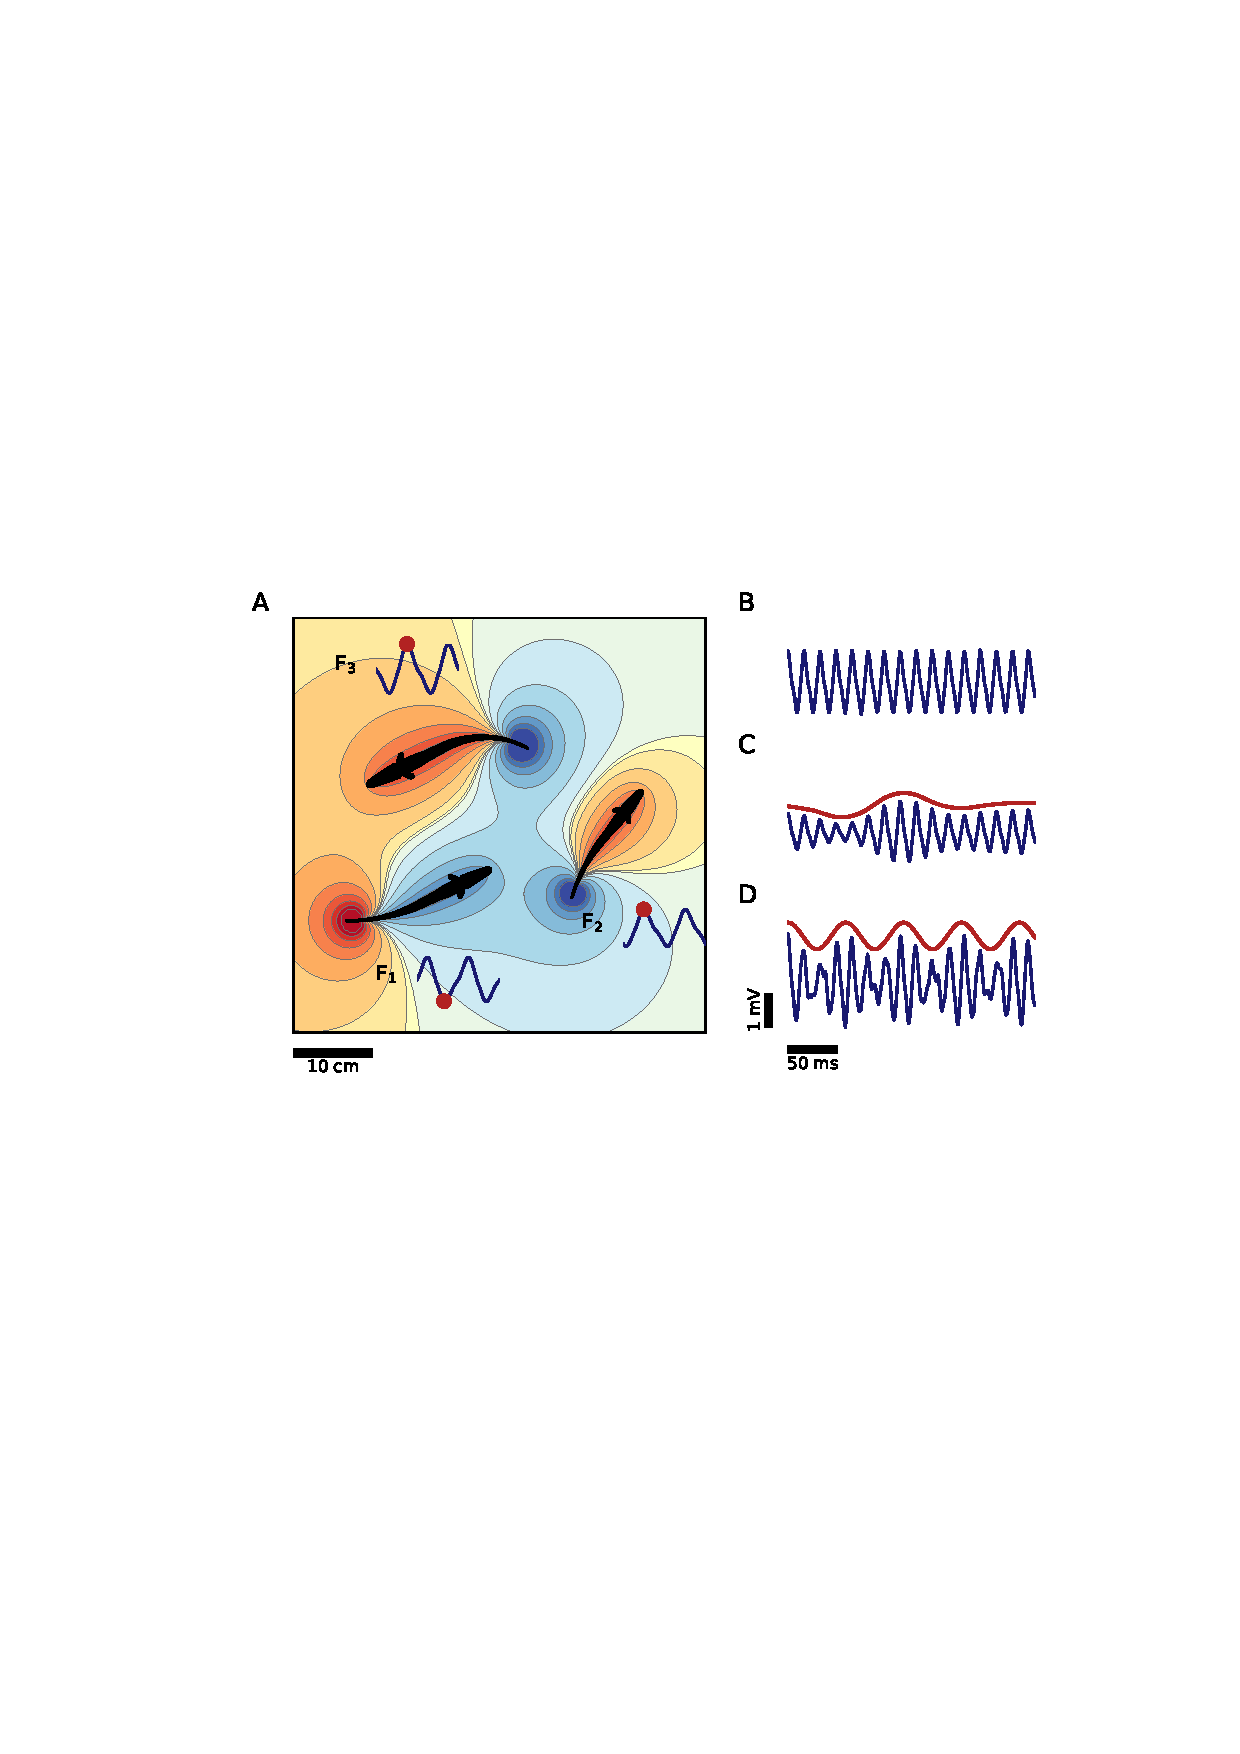
\includegraphics[width=0.7\linewidth]{figures/Fishies_cropped.pdf}
    \mycaption{Properties of the electric field in weakly-electric fish}{\textbf{A:} The fish surround themselves with a bipolar electric field. The superposition of electric fields alters their spatial properties. Thereby, the phase of the EOD influences the extend and direction of the electric field of each fish (red marker in EOD waveform). \textbf{B:} Quasi-sinusoidal waveform of the EOD of a single wave-type electric fish. \textbf{C:} Amplitude modulations (AM) of an individual fish recorded by external electrodes. The AM is caused by the movements of the fish relative to the recording electrodes. \textbf{D:} Amplitude modulation or beat caused by the superposition of two electric fields. The frequency of the beat is given by the difference in frequency between the individual fish (Figure from \cite{raab2022social}).}
    \label{fig:Electric fields}
\end{figure}

\subsection{The problem of detection}
For the exploration of the chirp function, two requirements have to be met. First, chirps need to be recorded to be analyzed in the first place. Secondly, the analysis depends on the ability to detect chirps in the recordings. Optimally, the method fulfilling these two requirements is suited for deployment in laboratory settings as well as in the field. Chirp recording is the least problematic part. As chirps alter the EOD$f$, they can readily be recorded by a pair of electrodes placed in the vicinity of the fish \parencite{bendaPhysicsElectrosensoryWorlds2020}. A common approach in laboratory settings is to simulate a conspecific with a pair of electrodes which should cause the recorded individual to chirp. These can then be recorded with a second pair of electrodes \parencite{zupanc1993evoked, hagedornCourtSparkElectric1985a, dunlapDiversityStructureElectrocommunication2003, englerSpontaneousModulationsElectric2000a}. However, the laboratory does not reflect the natural habitat of the animals since the behavioral context of chirps emitted in the wild is highly variable \parencite{henningerStatisticsNaturalCommunication2018}. Thus, there is a need of recording fish in their natural habitat while freely behaving and interacting with each other. This is why recently, research is more and more shifted to the field \parencite{henningerStatisticsNaturalCommunication2018, fugere2011electrical, zubizarreta2020seasonal}. With this increasing change in research approach, new methods that allow for the recording of multiple fish in the wild were required. One approach was developed by \textcite{henningerStatisticsNaturalCommunication2018} and successfully tested in Panama, where the authors simultaneously recorded multiple individuals of four species of weakly-electric fish. They used a grid-like array of at least 54 electrodes which was submerged at the cut bank side of a stream. Later, a refined version of the grid was applied for further recordings in Colombia \parencite{raab2022AdvancesNoninvasiveTracking}. As such, the recording problem has been solved for the laboratory as well as the natural setting. The detection of chirps, however, turned out to be the bigger problem. As part of successful detection, it is required to correctly identify the chirp in the EOD track as well as assign the individual chirp to the correct animal. This is particularly difficult in recordings of multiple fish because the detection of a chirp implies that the underlying EOD$f$ is tracked for every animal. One approach for the analysis of electric signals in weakly-electric fish are spectrograms (Fig. \ref{fig:introplot}). Since chirps are very fast changes in the EOD$f$, a sufficiently high resolution in the time domain is necessary to resolve them. But, an increase of the resolution in time is accompanied by a resolution decrease in the frequency domain, which renders the distinction of the EOD$f$s of the chirping fish impossible. Given the situation of two fish with a similar EOD$f$, and the individual with the lower frequency emitting a chirp, it is unfeasible to assign the chirp to the correct individual by only using the spectrogram. Thus, chirp detection is surely not a trivial problem. \textcite{raab2022AdvancesNoninvasiveTracking}, based on previous work by \textcite{henningerTrackingActivityPatterns2020}, developed an algorithm that solves one part of the issue. It is capable of extracting EOD tracks by using both the EOD$f$ in the spectrogram as well as the spatial distribution of EOD power across electrodes \parencite{raab2022AdvancesNoninvasiveTracking}. This way, it is possible to obtain the EOD track of individual fish in recordings with multiple fish in space and time (Fig. \ref{fig:introplot}). Only with this groundwork, it is achievable to detect chirps in the first place. 

\vspace{\baselineskip}

To overcome the remaining problem of chirp assignment, we refined previous work on this issue \parencite{henningerStatisticsNaturalCommunication2018}. In the following, we describe and test the first draft of a chirp detection algorithm capable of assigning chirps to individual fish in recordings with multiple animals. Our approach was to include a dynamic filter that searches for a frequency range between the individual EOD$f$'s free of interference. In a second step, we tested the algorithm with a data set obtained by \textcite{raabElectrocommunicationSignalsIndicate2021}. Thereby, individuals of the species \textit{Apteronotus leptorhynchus} were recorded while competing for a superior shelter in dyads. We were able to detect 25766 chirps in this data set alone and analyzed the context in which they were emitted. Thereby, we could not fully replicate suggestions for chirp function from the literature. However, some of our results indicate the association of chirps with a specific type of event during aggressive encounters.

\begin{figure}[H]
    \centering
    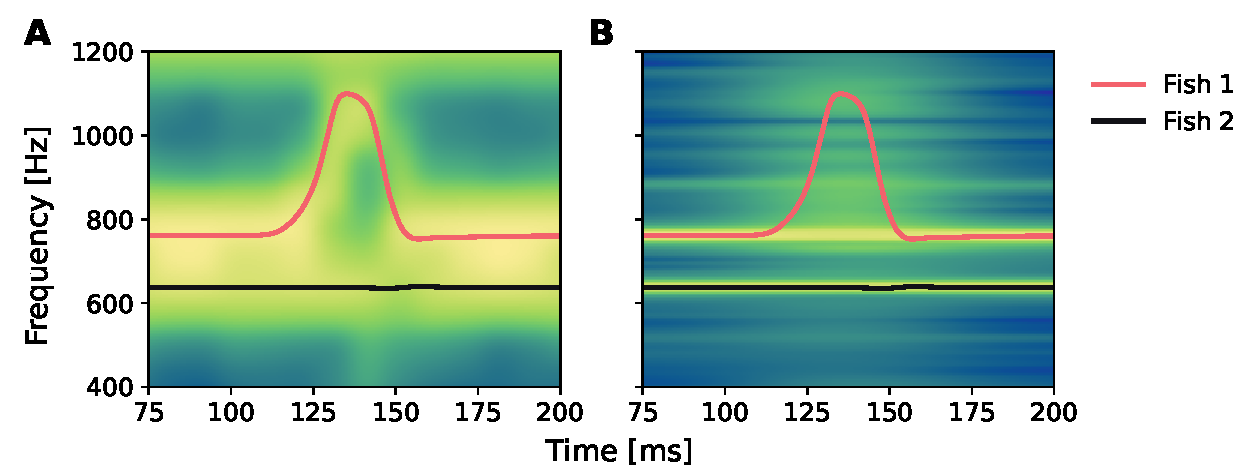
\includegraphics[width=1\linewidth]{figures/introplot.pdf}

    \mycaption{Spectrogram of signal containing the EODs of two fish.}{The line plots indicate the instantaneous frequency of the respective individual, which we obtained by filtering the signal around its frequency component. \textbf{A:} Fish 1 produces a chirp that is visible by the frequency excursion in the instantaneous frequency and spectrogram if the frequency resolution is sufficient (NFFT=133.3, 20\% overlap). \textbf{B:} If the frequency resolution is lower, fish can be distinguished in the spectrogram, but chirp detection and assignment are not reliable (NFFT=1333.3, 20\% overlap). }
    \label{fig:introplot}
\end{figure}

\todo[inline, color=orange]{Bilder von Lepto und seiner EOD waveform?}
\todo[inline, color=orange]{Messy in-text Quellen}
\todo[inline, color=orange]{Messy references Quellen}


\pagebreak
\section{Methods}
  \label{chap:methods}
  \subsection{Chirp detection algorithm}

We developed and tested the improved algorithm on the raw data from a competition experiment (more information in section \ref{Behaviour}, or in the Paper by \cite{raabElectrocommunicationSignalsIndicate2021}) with 15 electrodes arranged in a grid. To be able to analyze the communication signals of the fish, which are most prominently represented as changes in their EOD$f$, we used the frequency tracks that were already computed by \textcite{raab2022AdvancesNoninvasiveTracking}. A frequency track is an approximation of how the fundamental frequency of the EOD of a single fish evolves. But because they are estimated using a spectrogram, they lack the temporal information needed to resolve transient frequency changes of a chirp. For this reason, we use the raw data, which has the appropriate temporal resolution to resolve chirps. To extract the EOD of single individuals, the frequency tracks are used to build specific band pass filters for every fish. Because the baseline EOD$f$ of a single fish changes with temperature and communication signals, filtering had to be performed in time windows. Additionally, to obtain the best signal for a freely moving fish, we choose the electrode with the highest power for every single rolling window. For each time window, we extract the amplitude of the baseline, the instantaneous frequency, and the amplitude of the search frequency, which all change during the production of a chirp. Simultaneously detected peaks on all three features are classified as a chirp. All signal processing steps that the raw data in a single rolling window snippet goes through are summarized in figure \ref{fig:algorithm}. The following paragraphs describe the processing steps in the same order as they are organized in the code of the algorithm. 

\subsubsection{Loading and preparing the data set}

The parameters used by the algorithm are all adjustable using a \codeword{yaml} configuration file, which includes sections for the path to the data set as well as to the output directory. The program loads the raw data as well as the frequency tracks for every fish in the recording and generates time windows, in which it iterates across the raw data set. For each window in time, it iterates through the respective windows on the frequency tracks of all the fish in the recording. This approach is arguably less intuitive compared to iterating through the full time of the recording on the frequency track of a single fish and then skipping to the next individual. However, it reduces the number of times the more memory- and hence computationally demanding raw data set needs to be loaded. 

\subsubsection{Rolling windows and their overlap}

To reduce the edge effects caused by filtering, we overlapped the rolling windows (window duration of \SI{5}{\second}) by one second and discarded the first and last \SI{250}{\milli\second} of a single window. This resulted in a true overlap of \SI{0,5}{\milli\second} in which chirps might be detected twice. To resolve this issue, we grouped all chirps that occurred less than \SI{20}{\milli\second} apart from each other as a single chirp. 

\subsubsection{Following a fish through space}

The raw data set was recorded using an electrode grid. Hence, the EOD amplitudes of single fish varies between electrodes, because the amplitude decreases with the distance between an electrode and a moving fish. These changes in amplitude convey information on where the individual of interest is located in space. For optimal detection of chirps, we should use the strongest electrode for one fish, since it should have the highest signal-to-noise ratio. Additionally, if multiple fish are further apart, it is advantageous to use the electrode that is closest to one fish, but not the other, to increase the odds of correct sender assignment. For each iteration of the algorithm, we start off with a short (\SI{5}{\second}) snippets of the approximated frequency track and respective powers of the frequencies of an individual fish on the same temporal extent. To decide upon which raw data snippet for this fish across the pool of 15 electrodes the algorithm should load for optimal performance, we first had to determine, to which electrode the fish was the closest in the current window in time. To determine the best electrodes, we simply use the ones that had the highest power in the tracked frequencies, since power is proportional to the amplitude squared. In the current implementation, we repeat the following pipeline for the two electrodes with the highest power for the current fish of interest. 

\subsubsection{Feature extraction}

After determining the best electrodes, we load the raw data snipped for the respective time window. This results in a data set of the frequency track of a fish (Figure \ref{fig:algorithm}, A, red)  and the raw data (Figure \ref{fig:algorithm}, A, spectrogram), which the algorithm uses to extract more information. For each frequency track of an individual fish in each window, the raw signal \SI{5}{\hertz} is then band pass filtered with cut off frequencies above and below the baseline of the frequency track. This effectively provides an approximation of the recorded signal as if the current fish was the only one in the area. However fast frequency excursions, e.g. during chirps, are lost because they exceed the frequency limits of the cutoff frequencies. In other words, the peak of the chirp is filtered out by the band pass filter and that is why we see a trough in the amplitude. We use this to our advantage because the amplitude of the signal drops at theses points in time. To use the amplitudes of this signal, we extract the envelope using a low pass (cut off at \SI{25}{\hertz}) filter multiplied by the square-root of two (Figure \ref{fig:algorithm}, B, red). In addition to the amplitude trough, a chirp should also change the frequency of the signal, even if the actual peak gets lost due to filtering. To detect such transient frequency changes, we also compute the instantaneous frequency of the filtered baseline, which can be achieved by extracting the inverse of every single period using the zero crossings of the signal (Figure \ref{fig:algorithm}, B, orange).  But using just the envelope and the instantaneous frequency of the EOD baseline of the fish was not sufficient to determine whether the anomaly we detected is a chirp or is caused e.g. by the movement of the fish. To deal with this issue, we used the notion that chirps are always up-modulations of the frequency that reach values of +\SI{50}{\hertz} to +\SI{300}{\hertz} above the baseline EOD$f$ of the emitting fish \parencite{zakonEODModulationsBrown2002a}. The first approach by \textcite{henningerStatisticsNaturalCommunication2018} was to filter a band at approximately +\SI{10}{\hertz} above the baseline and look for peaks in the power of this filtered band. We call this area the 'search frequency'. However, this method comes with the limitation, that if there are multiple fish and one of them has a baseline EOD$f$ that is coincidentally higher than the frequency of the current analyzed fish, the search frequency will become unusable. If the search frequency is close to- or at the baseline frequency of a fish with higher EOD$f$, chirps from the fish with a lower EOD$f$ would not be correctly assigned to the sender (Figure \ref{fig:henninger}). We adopted the method first documented in \textcite{henningerStatisticsNaturalCommunication2018} but introduce a dynamically adjusted search frequency. In our version of the chirp detection algorithm, the search frequency is still confined to a region of +\SI{20}{\hertz} to +\SI{100}{\hertz} above the baseline. In contrast to \textcite{henningerStatisticsNaturalCommunication2018} in this window, the frequency tracks of all other individuals are evaluated to find a region with the largest frequency difference from all other individuals that is still within the usual frequency peaks of chirps. The search frequency is then extracted in this window. This should make chirp detection and, most importantly, correct assignment to the sender, possible with recordings that include multiple individuals (Figure \ref{fig:dynamic}). The search window chosen in the example in Figure \ref{fig:algorithm}, A is indicated by orange dashed lines on the spectrogram. The envelope of the search frequency is visualized by the orange line in panel B. 

\begin{figure}[H]
    \centering
    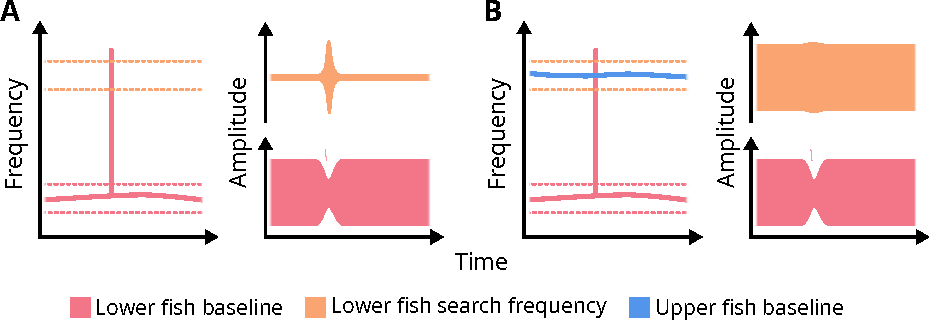
\includegraphics[width=\linewidth]{figures/henninger.pdf}
    \mycaption{Fixed search frequency}{Schematic sketch of a fixed search frequency used by \textcite{henningerStatisticsNaturalCommunication2018}. The search frequency is placed at a static \SI{10}{\hertz} above the baseline of the lower fish. \textbf{A:} If there is no upper fish with a higher EOD$f$ in the search frequency, a chirp detection can be implemented. The decrease in amplitude and the increase of amplitude in the search frequency can be used for the chirp detection algorithm. \textbf{B:}
    In the case that there is another fish with an EOD$f$ in the search frequency, chirp detection is impaired. The EOD at the search frequency contains the chirp of the lower fish and the EOD of the upper fish, which is making the detection of the chirp unreliable.}
    \label{fig:henninger}
\end{figure}

\begin{figure}[H]
    \centering
    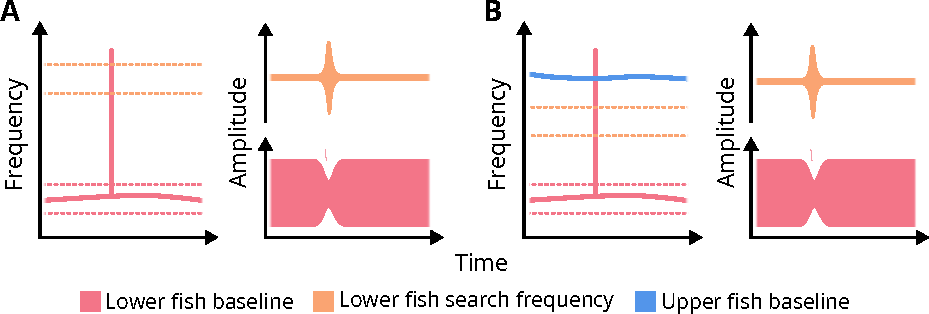
\includegraphics[width=\linewidth]{figures/dynamic.pdf}
    \mycaption{Dynamic search frequency}{Schematic sketch of a dynamic search frequency implemented in the new algorithm. The search frequency is dynamic in a range of \SIrange{20}{100}{\hertz} above the baseline of the lower fish. \textbf{A:} If there is no upper fish with a higher EOD$f$ in the search frequency, chirp detection can be implemented. The decrease in amplitude and the increase of amplitude in the search frequency can be used for the chirp detection algorithm. \textbf{B:}
    In the case that there is another fish with an EOD$f$ in the search frequency, the search frequency changes dynamically to a space with the largest difference to the upper fish. The chirp assignment is now possible with a correct sender assignment.}
    \label{fig:dynamic}
\end{figure}

\subsubsection{Feature processing}

The features we extracted, particularly the filtered baseline EOD, are also subject to change e.g. when the fish moves. But changes due to movements happen on a larger time scale. To reduce the impact of this noise, we additionally band-pass filtered the baseline envelope with cutoff frequencies \SI{2}{\hertz} (low-cutoff) and \SI{100}{\hertz} (high-cutoff). Additionally, we invert the baseline envelope to turn troughs into peaks for detection purposes. For the instantaneous frequency, we took the absolute and shifted it by the median of the EOD$f$ ($|EODf_{inst} - med({EODf_{inst}}|$). The instantaneous frequency during a chirp was negative in some cases. This irregularity is discussed in section \ref{ref:insta}. 
The search frequency required no additional processing. The processed features are visualized in the panel C of Figure \ref{fig:algorithm}. We then detected the peaks of all three features using a prominence threshold of 0.00005 for the baseline envelope, 0.000004 for the search frequency, and 2 for the instantaneous frequency.

\subsubsection{Peak classification}

Since all three features should coincide temporally with the peak in frequency during a chirp, the first criterion for a chirp was that peaks were detected on all three features simultaneously. More specifically, we chose \SI{20}{\milli\second} as a tolerance window where the peaks must co-occur. Additionally, since we repeated the algorithm on the two electrodes of the highest power for the current time window, we set a threshold of the number of electrodes on which the chirp must appear to be accepted as a chirp. In the current implementation, the chirp must be detected on just a single electrode. If a chirp is detected we compute the mean of the three time points on which the peaks were found and appended the resulting time stamp to the chirp times of the current fish.

\begin{figure}[H]
    \centering
    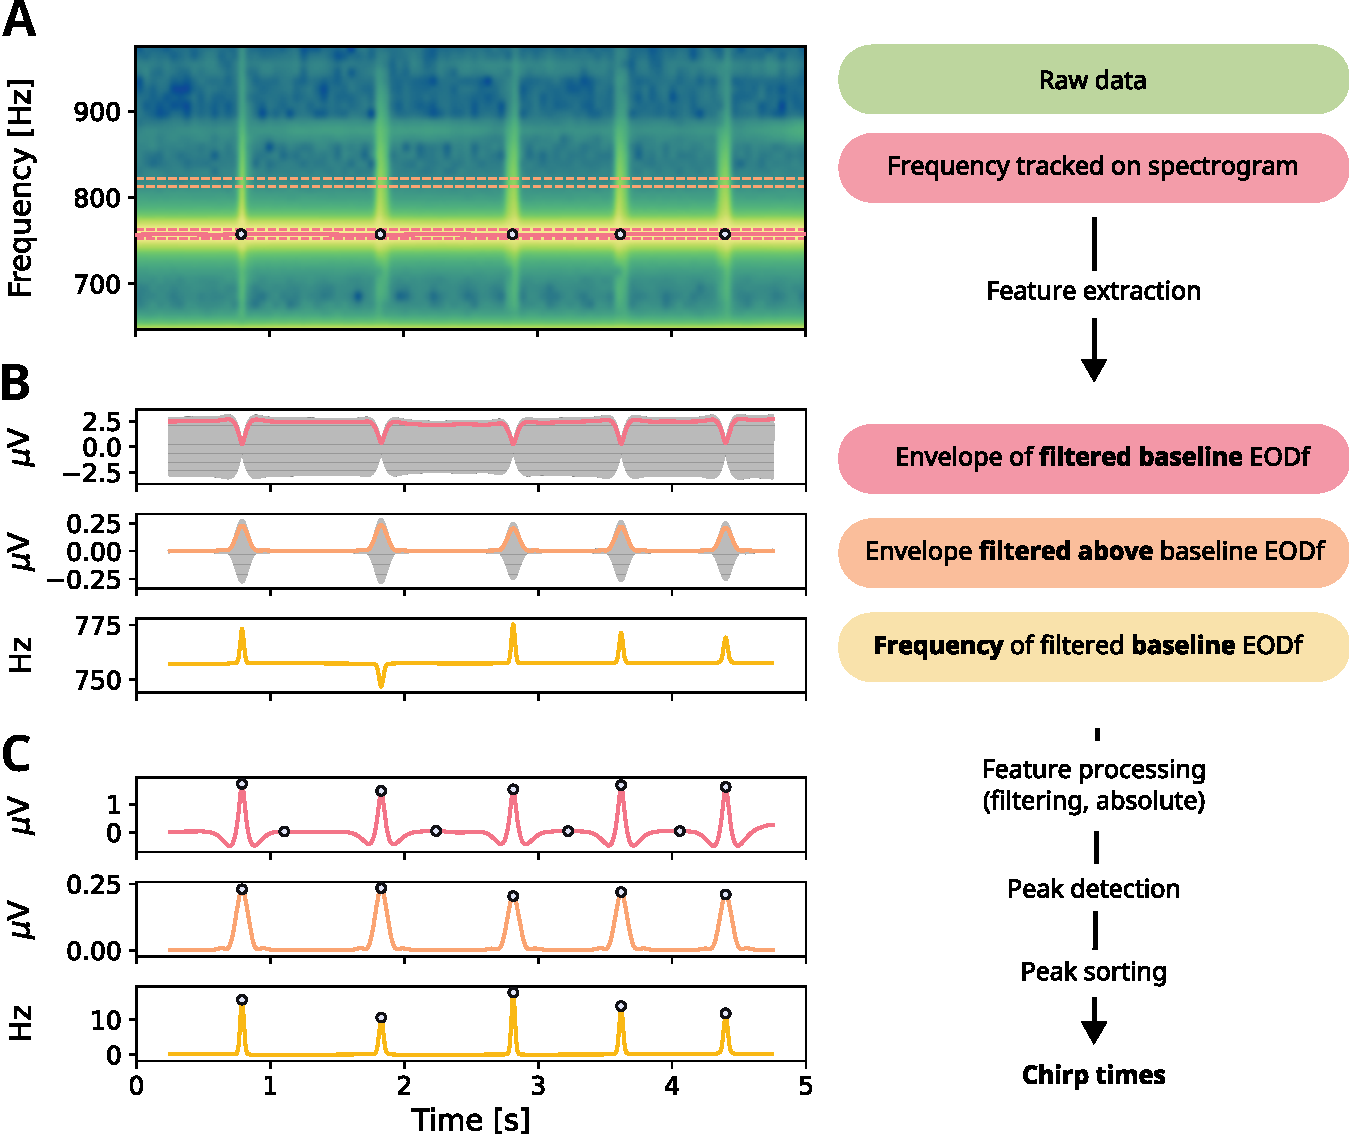
\includegraphics[width=\linewidth]{figures/10.0_11245.5.pdf}
    \mycaption{Core processing pipeline of the chirp detector.}{The left side shows how the data is modified while it passes the algorithm. The right side is color-coded with respect to the plots and indicates what kind of data is visualized and how it is processed. \textbf{A:} The spectrogram on the top is used to visualize the raw data. The red line on the spectrogram indicates the tracked frequency. \textbf{B:} The subplots show the three features that the algorithm extracts from the raw data using the frequency tracks of the individual fish. Red indicates the envelope of the baseline EOD$f$ for a single fish, which we obtain by filtering the raw signal around the tracked frequency. The envelope of the 'search frequency' we obtain by filtering a narrow band inside a dynamically adjusted window above the baseline EOD$f$ of the respective fish is indicated in orange. The search frequency band is also indicated by dashed lines in the same color on the spectrogram. The yellow line is the instantaneous frequency of the filtered baseline (red), which changes if the signal disappears out of the filtering window during a chirp. \textbf{C} illustrates how the three features appear after they are processed. The dots indicate the detected peaks. The dots on the spectrogram indicate the detected chirps after the peaks are sorted.}
    \label{fig:algorithm}
\end{figure}

\subsection{Behavioral data used to test the algorithm } \label{Behaviour}

We tested the algorithm on a data set published by \textcite{raabElectrocommunicationSignalsIndicate2021}. The dataset was recorded using 21 mature \textit{Apteronotus leptorhynchus} from a tropical fish supplier. 9 males and 12 females, all in non-breeding conditions, were used. The experiment was conceptualized to understand the role of rises, another communication signal, during the competition of two fish for a superior shelter. The experiments took place in a \SI{100}{\liter} tank with a superior shelter in the center surrounded by other, less optimal shelters. The bottom of the tank was equipped with 15 mono-polar electrodes with low-noise buffer headstages. A reference electrode was positioned in a corner of the tank. The electric signals were first amplified and then digitized at \SI{20}{\kilo\hertz} per channel. The movement of the fish was recorded by a video camera mounted above the aquarium. Behavior (chasing events and contacts) were annotated manually using the software package BORIS \parencite{https://doi.org/10.1111/2041-210X.12584}.

\subsection{Data analysis}

The chirp detection algorithm as well as our subsequent analysis were written in Python 3.10.9 using the packages numpy, scipy, matplotlib, \href{https://github.com/janscience/thunderfish}{thunderfish} and \href{https://github.com/janscience/audioio}{audioio} \parencite{2020SciPy-NMeth, Hunter:2007, harris2020array}. All scripts as well as the required package versions are publically available in a \href{https://whale.am28.uni-tuebingen.de/git/raab/GP2023_chirp_detection}{git repository} (\url{https://whale.am28.uni-tuebingen.de/git/raab/GP2023_chirp_detection}). The temporal relation between chirps and chasing events was analyzed using a cross-correlation analysis. We computed the temporal differences between agonistic events (chasing onset, -offset and contact) and the chirps up to $\pm$ \SI{90}{\second} before and after the event. We then convolved the temporal differences with a Gaussian kernel with a standard deviation of \SI{2}{\milli\second}. To generate a baseline to compare the convolution with we randomly shuffled the chirp intervals in 50 permutations and recomputed the convolution for each. The baseline distribution was then obtained by the median across the permutations with the 5th and 95th percentile respectively.

\pagebreak
\section{Results}
  \label{chap:results}
  \subsection{Chirps during dyadic competitions}

We used our algorithm to detect chirps in a dyadic competition experiment where two individuals competed for one superior shelter. In this exemplary recording almost all physical contacts, chasing events, and chirps happened during the dark phase of the experiment (Figure \ref{fig:timeline}, top rows in raster plot). We can estimate that the winner (yellow) did not chirp as much as the loser (red) of the competition. In this example, the winner emitted only 10 chirps whereas the loser produced close to 400 chirps(Figure \ref{fig:timeline}).
\begin{figure}[H]
    \centering
    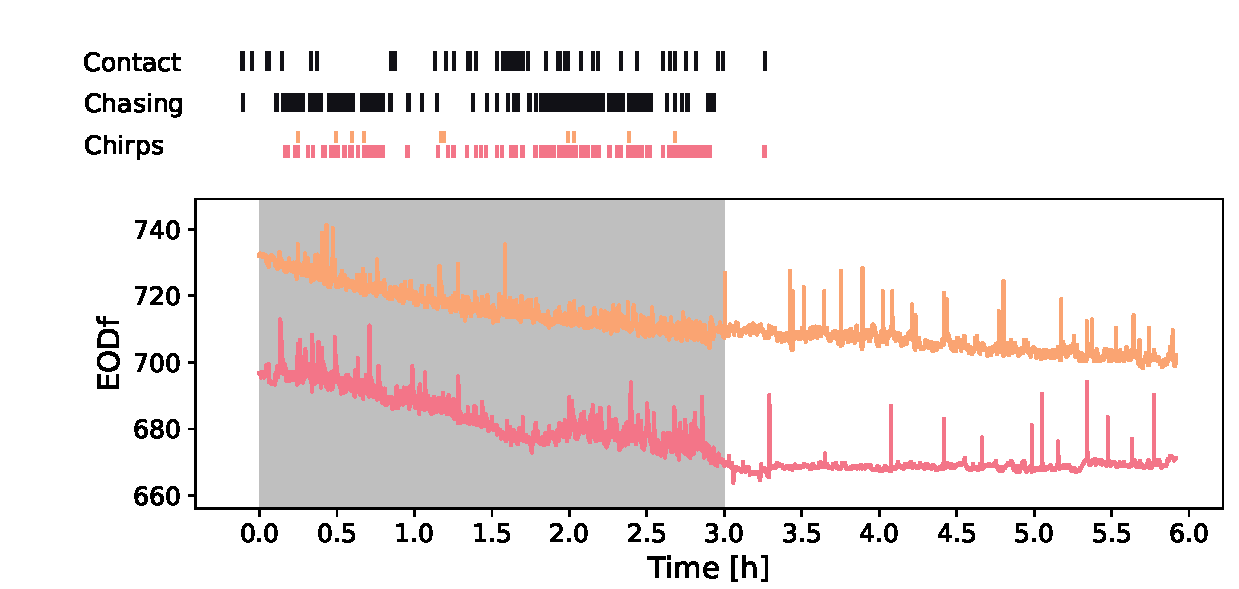
\includegraphics[width=\linewidth]{figures/timeline.pdf}
    \mycaption{Overview of a single trial of the competition experiment.}{The raster plots indicate the occurrence of the type of event. Rasterplots of chirps are color-coded with respect to the emitter of the chirp. The line plots indicate the EOD$f$ of the two fish over time as it was tracked on a spectrogram. Red was the winner of the competition, and yellow was the loser. The shaded area indicates the phase where lights were turned off.}
    \label{fig:timeline}
\end{figure}

Losers tended to chirp more than winners (Figure \ref{fig:winnerloser} A). This could be observed in 16 of the 22 valid trials (total n = 28) however this difference was not significant (Wilcoxon-test: z-statistic=67.0, pvalue=0.054). The outcome of the competition experiment was influenced by the size of the individuals. The winner of the dyadic interaction tended to have a greater size than the losers (Figure \ref{fig:winnerloser} B). For small size differences, there was an increase in chirp count, indicating that chirps increased in relevance for competition as the size difference decreased. The frequencies of the emitted EOD for winner and loser did not show any relevance for the outcome of the competition because the distribution for winner and loser is evenly spread over the range of EOD$f$ (Figure \ref{fig:winnerloser} C). 

\begin{figure}[H]
    \centering
    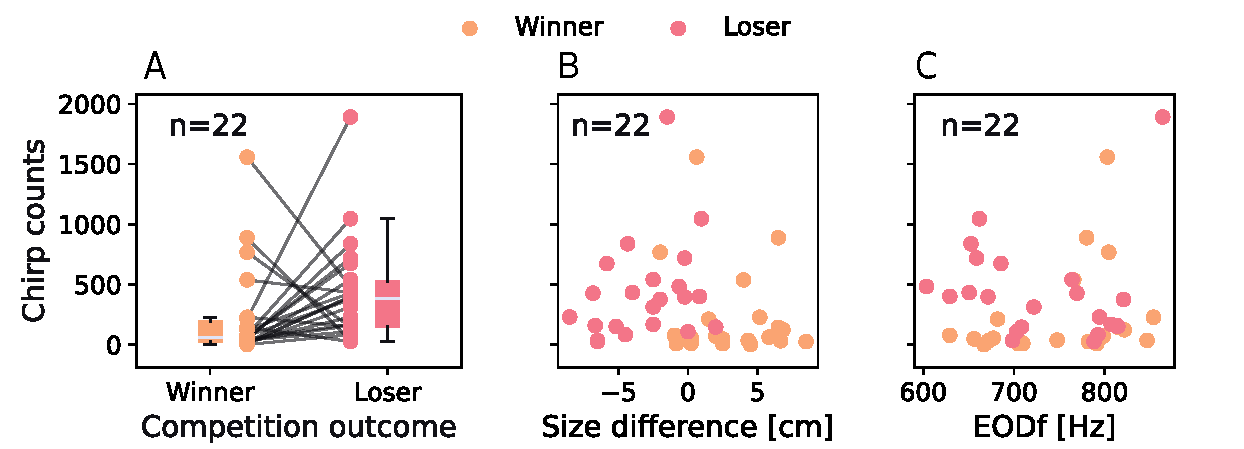
\includegraphics[width=\linewidth]{figures/chirps_winner_loser.pdf}
    \mycaption{Competition outcome }{compared to the emitted chirps in 22 valid parings (total n=28). \textbf{A:} Winner and loser of the competition experiment displayed with their quantity of chirps. Connecting lines indicate the pairing in the experiment. \textbf{B:} Winner and Loser compared to their size difference [cm] and the number of chirps they emitted. Losers (orange) are usually smaller than winners ($\Delta$ size $<$ 0) \textbf{C}: EOD$f$s [Hz] of the winner and loser compared to their quantity of chirps.}
    \label{fig:winnerloser}
\end{figure}

\subsection{Chirps emitted by loser fish might disrupt chasing events}

\begin{wrapfigure}{R}{0.6\textwidth}
\vspace{-1cm}
  \begin{center}
    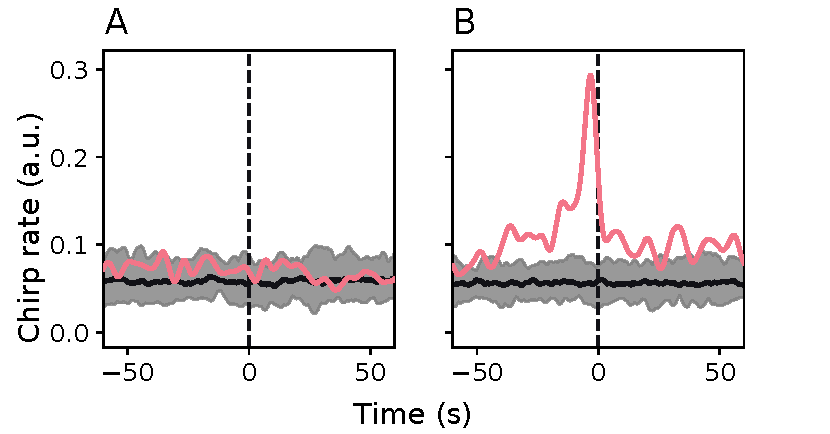
\includegraphics[width=\linewidth]{figures/kde.pdf}
    \end{center}
    \mycaption{Chasing-triggered chirps}{for two selected dyads. The time axis is centered around the offset of a chasing event. The black line indicates the bootstrapped baseline. The gray area is the bootstrapped confidence interval. The red line indicates the chirp rate estimated by a convolution with a Gaussian kernel. \textbf{A:} In most cases, there was no change in the chirp rate around an offset of a chasing event. \textbf{B:} But in a subset of the dataset chirping increased just before the chasing stopped.}
    \label{fig:kde}
\end{wrapfigure}

Losers tending to chirp more often than winners already hints towards a behavioral significance to chirps during competitions. We evaluated the temporal correlation of chirps and agnostic behaviors to further investigate the behavioral significance of chirps in dyadic encounters. For this, we computed the chasing-triggered chirp rate of the on- and offset of chasing events and contacts. The chasing-triggered chirp rate consists of chirps centered around agonistic events. After this sorting, we estimated the distribution of chirps for the events using a convolution with a Gaussian kernel. We focused on the offset of chasing events because the onset and physical contact did not show consistent increases in chirp rate. For approximately a third of all dyadic competitions, there was an increase in chirp rate before the offset occurred (Figure \ref{fig:kde} right). In the other cases, there was no interaction of the offset and chirps (Figure \ref{fig:kde} left). This was compared to a permutated baseline to show a significant increase in chirp rate. The summarized chirp rates across all competitions did not show an increase in chirp rate around the offsets of the chasing events.

\newpage
\FloatBarrier
\begin{wrapfigure}[14]{hr}{0.4\textwidth}
    \centering
    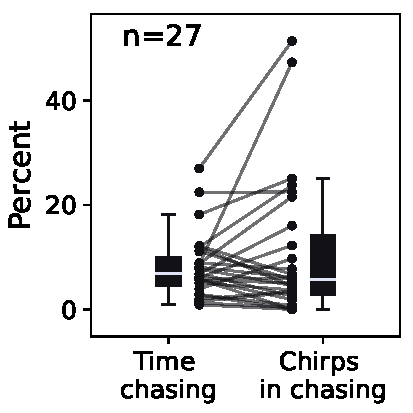
\includegraphics[width=\linewidth]{figures/chirps_in_chasing.pdf}
    \mycaption{Proportion of time spent and chirps emitted in chasing events.}{Relative time spent of the dark recording phase (3 h) in chasing events for single trials (\textbf{left}) and the relative quantity of chirps that were emitted during a chasing event for each recording (\textbf{right}). The lines show that the proportion of chirps during chasing events was only elevated for a subset of the competitions.}
    \label{fig:chasing}
\end{wrapfigure}
\FloatBarrier

To summarize this, we compared the percentage of time spent in chasing events with the percentage of chirps emitted in chasing events. This comparison should indicate that when the two fish are in a chasing event, and the chirps are used to carry information specifically related to competition, there should be an increase in the percentage of chirps in these chasing events. In 15 out of 27 pairings the percentage of time spent in chasing events was higher than the percentage of chirps emitted during chasing, showing that chirps may not be used for transferring information about their physical status in those cases. This indicates that chirps are not specifically used for the offset of chasing events because their percentage of occurrences is often lower than the time spent in these chasing events. 


\pagebreak
\section{Discussion}
\label{chap:discussion}

We detected 25766 chirps in this dataset which included 27 valid trials of recordings that lasted 6 hours each. The number of detected chirps is close to the currently largest reported dataset by \textcite{obotiWhyBrownGhost2022} which contains multiple different experiments. This was achieved by extending the chirp detection algorithm by \textcite{henningerTrackingActivityPatterns2020}. We added a dynamic search frequency and combined peaks of the envelope in the EOD amplitude, the envelope of the dynamic search frequency, and the instantaneous frequency for chirp detection. The chirps we detected on a dataset published by \textcite{raabElectrocommunicationSignalsIndicate2021} indicate that individuals that win the competition for a superior shelter chirp less than the losers. Moreover, in some of these pairings, chirps emitted by the loser are temporally correlated with the offset of an agonistic interaction. This indicates, that chirps might be used by losers to terminate chasing events.

\subsection{Assessing detection performance}

While our chirp detector detected many chirps, the performance of the algorithm was not quantified yet. We only used a small trial dataset to visually asses whether chirps are detected or not. Additionally, the EOD$f$ of the fish in the trial data set were rather far apart, making it easy to correctly assign chirps. To assess the performance of our analysis data set, we visually inspected each iteration of the algorithm (in 5 seconds snippets) for one whole recording. However, for future uses of this detector, it is imperative to quantify the detection performance and tune the parameters accordingly. This is especially important considering that the main innovation of this algorithm is not to detect but to correctly assign chirps. We predict that the performance in the correct assignment will most likely drop with decreasing difference frequencies. If this is the case we have to quantify this parameter as well. In conclusion, future work on this algorithm should include a synthetic data set that reflects the natural variability to quantify the detection performances of multiple chirp detection parameters.

\subsection{The problem of normalization}

Currently, a major flaw of the chirp detector is that the peak detection parameters are fixed for each feature, and decided upon by trial and error. We reached the most error-free performance with high thresholds. A side effect is that the great majority of the chirps are only detected on a single electrode. If chirps would be detectable on multiple electrodes, the smallest number of electrodes on which a chirp must be detected could be used as an additional detection parameter. But to do this, ideally, we would need to be able to use the same peak detection parameters across all electrodes and for all features. And to achieve this we should normalize our feature arrays not only across features but also across electrodes. The difficulty with normalization arises with the rolling windows and the changing electrodes. If there is no chirp in a certain window, normalizing across electrodes over just that window would scale up all noise so that the peak detector would find many peaks. Most of the time
 these peaks do not occur at the same time and thus are not falsely detected as chirps, but sometimes, they are. The current method to fix this is to not normalize at all and hard-code peak detection thresholds. This solution is not flexible and might fail completely for new data sets without manually adjusting the parameters. The seemingly easy approach would be to save the data of all feature arrays for each iteration to disk and normalize across all data before running the chirp detector. But the fact that for each iteration we jump between electrodes makes this step complicated and impractical. Another approach could be, to determine 'chirp-less' windows by a single parameter before normalization. If e.g. there in no peak in the search frequency, we could just skip to the next window instead of running the whole detection routine. Normalization could then be performed only in windows that have a peak in search frequency. 

\subsection{Why can the instantaneous frequency go down during a chirp?} \label{ref:insta}

While computing the instantaneous frequency we often encountered troughs instead of peaks in frequency during chirps. We simply circumvented this issue by taking the absolute of this instantaneous frequency. This phenomenon is critical because chirps are defined by a positive frequency excursion and not by a decrease in frequency. This decrease was only found after we computed the band pass filter which is filtering \SI{5}{\hertz} around the baseline of the EOD$f$ of the individual fish. If we band pass-filtered in a way so that the chirp was still included in the signal, all peaks in the instantaneous frequency were positive. This indicates that the narrow band pass filter around the signal is causing these frequency drops. One explanation for this issue could be the reduced amplitude during a chirp. The band pass filter removes the high frequency components that a chirp introduces. If the amplitude reduction is high enough, the frequency information shifts to noise.  If this noise has only low frequency components the instantaneous frequency drops. If the chirp contrast is low and the amplitude of the baseline does not decrease strongly, the increase in frequency that is common during a chirp might be reflected in a peak. But if the contrast is high and the amplitude in the baseline breaks down this would reflect in a trough in the instantaneous frequency. Against this theory stands the fact that we observed the troughs in frequency in cases where the amplitude of the baseline did not break down strongly. 

\vspace{\baselineskip}

Another explanation are the properties of the band pass filter which can introduce a phase shift while the fish emits chirps. If the phase is shifted backward the frequency temporarily increases, and vice versa for forward phase shifts. We still do not fully understand this change in frequency yet. Further analysis should include plotting the transfer function of the filter since narrow pass bands could introduce anomalies. Additionally, we would like to simulate chirps with different parameters, such as chirp phase, height, width, and contrast to understand which parameters might result in a trough of the instantaneous frequency.

\subsection{Losers chirped more than winners}

The detected chirps in this experiment indicate that winners chirped less than losers in this competition experiment. We can hypothesize that chirps are used as a submissive signal conveying information about the physical condition \parencite{davies1978deep}, and therefore can settle the competition without fights that escalate. 
This result shows similarities to rises, another signal variation used by \textit{Aperonotus leptorhynchus}. \textcite{raabElectrocommunicationSignalsIndicate2021} showed that the loser of a competition experiment emitted more rises than the winner of the competition. Furthermore, the outcome of the competition is influenced by the body size: A larger body size is a predictor for winning the competition for the shelter \parencite{raabElectrocommunicationSignalsIndicate2021}. The frequencies of the individuals, on the other hand, do not seem to play a role in the outcome of the competition experiment. This needs to be further analyzed because the EOD$f$ is sexually dimorphic \parencite{meyer1987hormone}, and we did not take the sex of the pairings into account for our analysis.  

\subsection{Why chirps might only terminate chasing in some dyads}

Our results indicated that chirps can terminate chasing, hence we computed the chirp rate to the chasing on- or offset and physical events. Only for the chasing offset we could find a connection for some pairings in the competition experiment in a way that the chirp increases right before the offset of the chasing event. \textcite{raabElectrocommunicationSignalsIndicate2021} showed that rises are used by the subordinate to motivate mutual assessment. In the few cases where we observed increasing chirp frequencies at the offset of a chasing event, chirps may have been used by the loser of the competition to signal submission. Still, the mean for all pairings did not show a correlation of chirps and the chasing offsets. This can be explained by not including factors like sex and size difference in our analysis. The sex of the fish has an important role for the communication behavior in the mating season, where, the female emits a big chirp to signalize the spawning \parencite{hagedornCourtSparkElectric1985a, henningerStatisticsNaturalCommunication2018}. The size difference is also important for the outcome of the competition experiment, so there may be a link between the increase of chirping behavior and the offset of the chasing events with the size difference. This should be dissected further in the analysis of the behavioral data set. 

\subsection{Summary}

In conclusion, we were able to build the first chirp detector that might be usable on large data sets including multiple and freely moving individuals. Chrips can be detected by combining features from the changes in amplitude, instantaneous frequency, and a dynamic search window that is above the fish's own EOD$f$. We tested this detector on a data set of a competition experiment. We found that more chirps are produced when the size difference between the individuals was small and that the subordinates sometimes drastically increase their chirp frequency before a chasing event ends. This is the first step towards analyzing chirp-correlated behaviors in complex laboratory or field recordings to gain a clearer picture of the potentially multiple meanings of chirps. These first observations could inspire hypotheses that can then be verified in controlled experiments. 

\pagebreak
\printbibliography 
%\pagebreak
%\section{Appendix}
%  \label{chap:appendix}
%  \input{chapters/appendix.tex}

% Append pdf outputs from other programs to the document
% \includepdf[pages=-]{appendix/ab.pdf}
% \includepdf[pages=-]{appendix/cd.pdf}
% \includepdf[pages=-]{appendix/ef.pdf}

\end{document}